%%\title{EALIGN}
%  Changed by: Hans Grote, 13-Sep-2000 
%  Changed by: Werner Herr, 19-Jun-2002 
%  Changed by: Hans Grote, 19-Jun-2002 
%  Changed by: Werner Herr, 24-Jul-2002 
%  Changed by: Werner Herr, 02-Sep-2002 
%  Changed by: Hans Grote, 25-Sep-2002 

\section{Alignment Errors} %EALIGN: Define Misalignments} 
Alignment errors are defined by the EALIGN command. The misalignments
refer to the \href{../Introduction/local_system.html}{local reference
  system} for a perfectly aligned machine. Possible misalignments are
displacements along the three coordinate axes, and rotations about the
coordinate axes. Alignment errors can be assigned to all beam elements
except drift spaces. The effect of misalignments is treated in a linear
approximation. A \href{read HREF=../Introduction/monitors.html}{Beam
  position monitor} can be given read errors in both horizontal and
vertical planes. Monitor errors (MREX, MREY, MSCALX and MSCALY) are
ignored for all other elements. Each new EALIGN statement replaces the
misalignment errors for all elements in its range, unless
EOPTION,ADD=TRUE has been entered.  

Alignment errors are defined by the statement 

\begin{verbatim}
SELECT,FLAG=ERROR,RANGE=range,CLASS=name,PATTERN=string;
EALIGN, DX=real,DY=real,DS=real, 
        DPHI=real,DTHETA=real,DPSI=real, 
        MREX=real,MREY=real,
        MSCALX=real,MSCALY=real,
        AREX=real,AREY=real;
\end{verbatim}
and elements are now selected by the
\href{../Introduction/select.html}{SELECT} command. 

The attributes are: 
\begin{itemize}
\item DX: The misalignment in the \textit{x}-direction for the entry of the beam element (default: 0 m). 
\\ DX$>$0 displaces the element in the positive \textit{x}-direction 

\item DY: The misalignment in the \textit{y}-direction for the entry of the beam element (default: 0 m). 
\\ DY$>$0 displaces the element in the positive \textit{y}-direction 

\item DS: The misalignment in the \textit{s}-direction for the entry of the beam element (default: 0 m). 
\\ DS$>$0 displaces the element in the positive \textit{s}-direction 

\item DPHI: The rotation around the \textit{x}-axis. 
\\ A positive angle gives a greater \textit{x}-coordinate for the exit than for the entry (default: 0 rad). 

\item DTHETA: The rotation around the \textit{y}-axis according to the right hand rule (default: 0 rad). 

\item DPSI: The rotation around the \textit{s}-axis according to the right hand rule (default: 0 rad). 

\item MREX: The horizontal read error for a monitor. This is ignored if the element is not a monitor 
\\ If MREX$>$0 the reading for \textit{x} is too high (default: 0 m). 

\item MREY: The vertical read error for a monitor. This is ignored if the element is not a monitor 
\\ If MREY$>$0, the reading for \textit{y} is too high (default: 0 m). 

\item AREX: The misalignment in the \textit{x}-direction for the entry of an aperture limit (default: 0 m). 
\\ AREX$>$0 displaces the element in the positive \textit{x}-direction 

\item AREY: The misalignment in the \textit{y}-direction for the entry of an aperture limit (default: 0 m). 
\\ AREY$>$0 displaces the element in the positive \textit{y}-direction 

\item MSCALX: The relative horizontal scaling error for a monitor. This is ignored if the element is not a monitor. 
\\ If MSCALX$>$0 the reading for \textit{x} is too high (default: 0). A value of 0.5 implies the actual reading is multiplied by 1.5. 

\item MSCALY: The relative vertical scaling error for a monitor. This is ignored if the element is not a monitor.  
\\ If MSCALY$>$0 the reading for \textit{y} is too high (default: 0). A value of -0.3 implies the actual reading is multiplied by 0.7. 
\end{itemize}

Examples: 
\begin{verbatim}
SELECT, FLAG = ERROR, CLASS = MQ;                  
EALIGN, DX = 0.002, DY = 0.0004*RANF(), DPHI = 0.0002*GAUSS();
\end{verbatim}
Assigns alignment errors to all elements of class MQ.           



\begin{verbatim}
SELECT, FLAG = ERROR, PATTERN = "QF.*";            
EALIGN, DX = 0.001*TGAUSS(2.5), DY = 0.0001*RANF();
\end{verbatim} 
Assigns alignment errors to all elements starting with "QF". TGAUSS(2.5) means a Gaussian distribution cut at 2.5 sigma. 


%\href{xsdisp}{
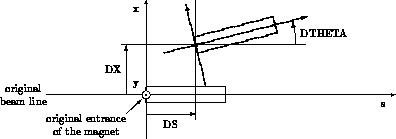
\includegraphics{figures/xs_align.png}

\textbf{Figure 1:} Example of Misplacement in the (\textit{x, s})-plane. 

%\href{xydisp}{
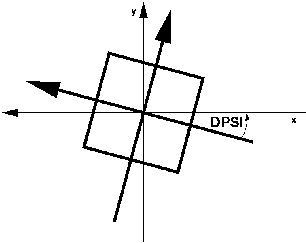
\includegraphics{error/dpsi.png}

\textbf{Figure 2:} Example of Misplacement in the (\textit{x, y})-plane. 

%\href{ysdisp}{
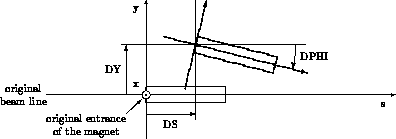
\includegraphics{figures/ys_align.png}

\textbf{Figure 3:} Example of Misplacement in the (\textit{y, s})-plane. 

%\href{monitor}{
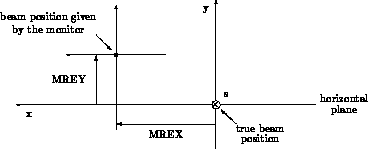
\includegraphics{figures/monitor_read.png}

\textbf{Figure 4:} Example of Read Errors in a monitor 

%\href{http://consult.cern.ch/xwho/people/1808} {Last updated:} 02.9.2002 \\ 
%\href{http://consult.cern.ch/xwho/people/1808}{Werner Herr} 18.6.2002 
